\documentclass[dvipdfmx]{jsarticle}


\usepackage{tcolorbox}
\usepackage{color}
\usepackage{listings, plistings}

%% ノート/latexメモ
%% http://pepper.is.sci.toho-u.ac.jp/pepper/index.php?%A5%CE%A1%BC%A5%C8%2Flatex%A5%E1%A5%E2

% Java
\lstset{% 
  frame=single,
  backgroundcolor={\color[gray]{.9}},
  stringstyle={\ttfamily \color[rgb]{0,0,1}},
  commentstyle={\itshape \color[cmyk]{1,0,1,0}},
  identifierstyle={\ttfamily}, 
  keywordstyle={\ttfamily \color[cmyk]{0,1,0,0}},
  basicstyle={\ttfamily},
  breaklines=true,
  xleftmargin=0zw,
  xrightmargin=0zw,
  framerule=.2pt,
  columns=[l]{fullflexible},
  numbers=left,
  stepnumber=1,
  numberstyle={\scriptsize},
  numbersep=1em,
  language={Java},
  lineskip=-0.5zw,
  morecomment={[s][{\color[cmyk]{1,0,0,0}}]{/**}{*/}},
  keepspaces=true,         % 空白の連続をそのままで
  showstringspaces=false,  % 空白字をOFF
}
%\usepackage[dvipdfmx]{graphicx}
\usepackage{url}
\usepackage[dvipdfmx]{hyperref}
\usepackage{amsmath, amssymb}
\usepackage{itembkbx}
\usepackage{eclbkbox}	% required for `\breakbox' (yatex added)
\usepackage{enumerate}
\usepackage[default]{cantarell}
\usepackage[T1]{fontenc}
\fboxrule=0.5pt
\parindent=1em

\makeatletter
\def\verbatim@font{\normalfont
\let\do\do@noligs
\verbatim@nolig@list}
\makeatother

\begin{document}

%\anaumeと入力すると穴埋め解答欄が作れるようにしてる。\anaumesmallで小さめの穴埋めになる。
\newcounter{mycounter} % カウンターを作る
\setcounter{mycounter}{0} % カウンターを初期化
\newcommand{\anaume}[1][]{\refstepcounter{mycounter}{#1}{\boxed{\phantom{aa}\textnormal{\themycounter}\phantom{aa}}}} %穴埋め問題の空欄作ってる。
\newcommand{\anaumesmall}[1][]{\refstepcounter{mycounter}{#1}{\boxed{\tiny{\phantom{a}\themycounter \phantom{a}}}}}%小さい版作ってる。色々改造できる。

%% 修正時刻: Sat Oct 30 09:03:09 2021


\section{コマンドプロンプトとは?}

\subsection{起動}

``スタートボタン'' -- ``Windowsシステムツール'' の中に ``コマンドプロンプト'' はある。

右クリックして、``スタートパネルにピン留めする'' かあるいは、``その他''
-- ``タスクバーにピン留めする'' にしておくとよい。

しかし、ふつうは以下の方法で起動する。

\begin{itemize}
 \item スタートボタン横の検索で ``cmd'' と入力して $<$Enterキー$>$
 \item エクスプローラのURL欄にて ``cmd'' と入力して $<$Enterキー$>$
\end{itemize}

\vspace{3mm}
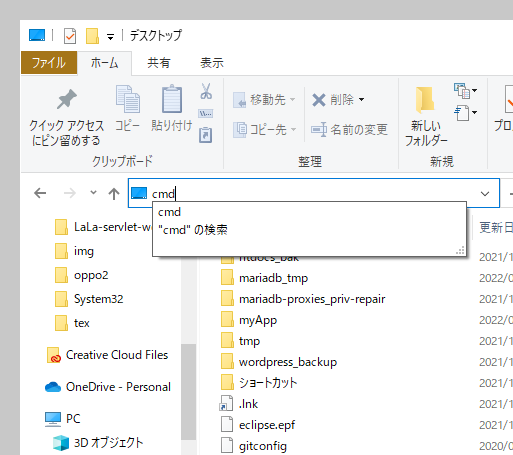
\includegraphics[width=10cm]{img/cmd-00-01.png}

これは、エクスプローラのURL欄に ``cmd'' と入力したところ。


\vspace{3mm} 
黒いウィンドウが表示される。これがコマンドプロンプト。

\newpage
\subsection{設定}

ウィンドウ左上のアイコンをクリックすると ``プロパティ''という項目がある。
それを選択すると、設定画面になる。

\vspace{3mm}
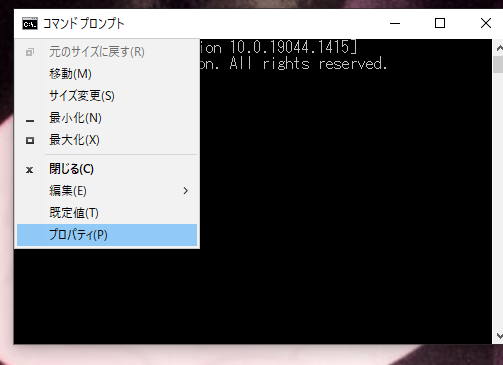
\includegraphics[width=8cm]{img/cmd-00-02.png}

これは、プロパティを選択しているところ。


\vspace{3mm}
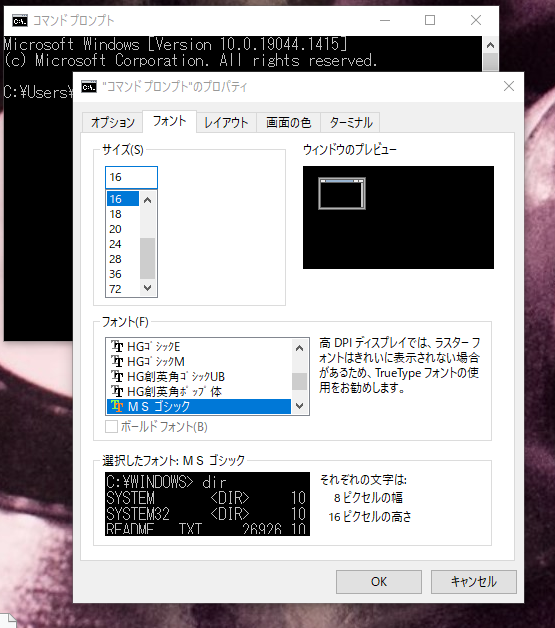
\includegraphics[width=8cm]{img/cmd-00-03.png}

これは、プロパティでフォントを選択しているところ。

\newpage
\subsection{動作を試す}

画面には、以下のような文字が表示されている。

\vspace{3mm}
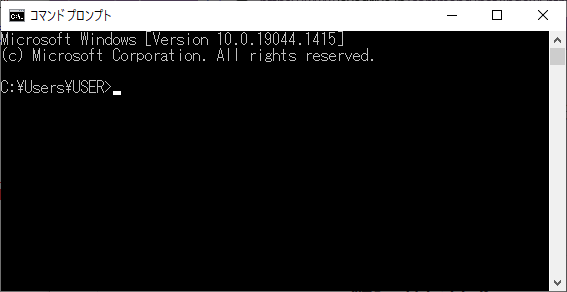
\includegraphics[width=12cm]{img/cmd-01.png}
\vspace{3mm}


\fbox{C:\\Users\\User$>$} はプロンプトといい、現在の位置を
ユーザーに示している。
また、$>$ という文字列に続けて文字を入力できることを示している。



試しに以下のコマンドを入力して $<$Enterキー$>$ を押してみる。

\fbox{ver}

\vspace{3mm}
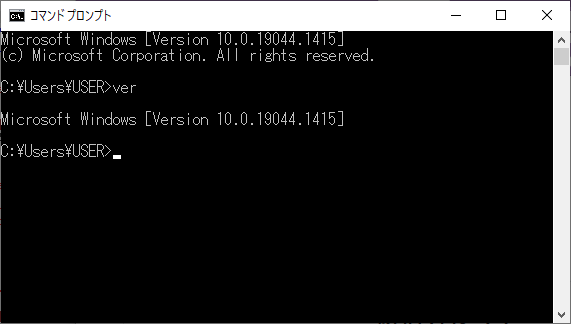
\includegraphics[width=12cm]{img/cmd-02-ver.png}
\vspace{3mm}

Windowsのバージョンが表示される。

今度は以下のコマンドを入力する。($<$Enterキー$>$も)

\fbox{date}

現在の日付が表示されて、次の行で
``新しい日付を入力してください: (年-月-日)``
と表示されて、入力が促される。

何も入力せず、そのまま $<$Enterキー$>$ を押せばよい。

\vspace{3mm}
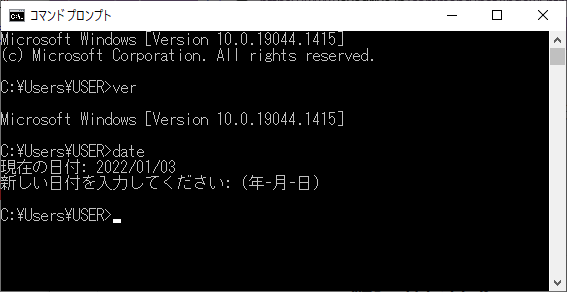
\includegraphics[width=12cm]{img/cmd-03-date.png}
\vspace{3mm}

\subsection{コマンドプロンプトとは?}

コマンドプロンプトというのは、この黒い画面に文字(コマンド)を入力して
コンピュータからの返答を得るというものである。

つまり、コンピュータとの「対話」である。
コンピュータと「チャット」しているようなものである。

コンピュータには二つの種類のアプリケーションがある。

\begin{itemize}
 \item GUIアプリケーション --- マウスで操作するアプリケーション
 \item CUIアプリケーション --- キーボード入力で操作するアプリケーション
\end{itemize}
\begin{flushright}
GUI --- Graphical User Interface \\
CUI --- Character User Interface
\end{flushright}



``WORD''などのアプリは GUIである。大半のアプリが GUI である。

しかし、CUIアプリも数多くある。特にプログラミング言語(PHP、Javaなど)は CUI である。

しかし、CUIだと使いづらいので、Javaでは Eclipse などの統合開発環境(IDE)
を使った開発が行なわれている。

先程の''ver''というのは、ひとつのアプリケーションで、``date''というのも
アプリケーションである。

``help''と入力すれば、コマンド(アプリ)の一覧が表示される。中にはシステムの改変を行うコマンドもあるので、表示されたコマンドを不用意に実行してはいけない。


\subsection{バッチファイル}

今作成した ``hello.bat'' はバッチファイルと呼ばれるもので、
コンピュータに与えるコマンドを手順として多数記述しておいて、
それらを実行させるものである。``スクリプト''とも呼ばれる。

今作成したのは簡単な手順であるが、業務で使われる場合は
複雑なものとなる。

拡張子は ``.bat''である。

``echo off'' は、コマンド文字列を画面に表示させないためのものである。
``@'' は、そのコマンドを画面に表示させないためのものである。




\section{コマンドプロンプトによるディレクトリ(フォルダ)の移動}

コマンドプロンプトには「現在の位置」が表示される。
「現在どの位置にいるのか」を理解する必要がある。

スタート・メニューからコマンドプロンプトを起動した場合、

\fbox{C:\yen Users\yen user} と表示される。
この場所を \textgt{ホームディレクトリ} あるいは \textgt{ホームフォルダ}
という。

また、この ``C:\yen Users\yen user'' を \textgt{パス} という。

この場所で \fbox{dir} とすると、この場所にあるファイルやディレクトリ(フォルダ)の一覧が表示される。

\vspace{3mm}
\begin{tabular}{|l|} \hline
Desktop --- デスクトップ \\
Documents --- ドキュメント \\
Downloads --- ダウンロード \\
Music --- ミュージック \\
Pictures --- ピクチャ \\
Videos --- ビデオ \\ \hline
\end{tabular}
\vspace{3mm}

\fbox{dir \ /w}

とすると、横に広げてディレクトリ(フォルダ)の状態を一覧できる。


たとえば、デスクトップ に移動するには、\fbox{cd \ desktop} とする。

\fbox{dir} とすると、たくさんのファイルやフォルダがあるので、
画面の上に過ぎ去ってしまう。
そこで、以下のようにする。

\fbox{dir \ /p}

すると、1画面分ごとに表示される。
そのとき、一番上には、以下のように表示される。

\vspace{3mm}
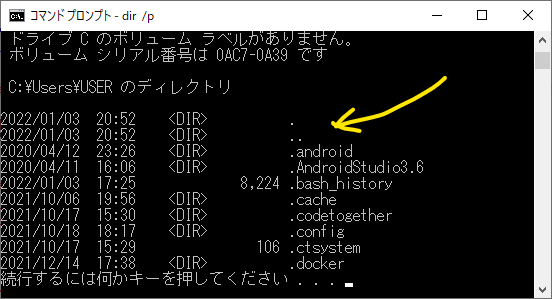
\includegraphics[width=10cm]{img/cmd-06-dir.png}
\vspace{3mm}

この \fbox{.} は、「ここ」をあらわす。

\fbox{..} は、「ひとつ上」をあらわす。

だから、``./memo.txt''とすると、このディレクトリ(フォルダ)にある memo.txt
のことになる。(memo.txtが存在するとして)

また、``../some.txt'' とすると、ひとつ上のディレクトリ(フォルダ) にある
some.txt ということになる。(some.txtが存在するとして)

さらに \fbox{cd \ ..} とすると、ひとつ上のディレクトリ(フォルダ)に移動できる。


\section{システム環境変数の PATH への登録}

テラパッドを起動するには、デスクトップのテラパッド・アイコンをダブルクリックするとか、
メニューから起動するとかしなければならない。

先ほどのコマンドプロンプトにて、\fbox{ terapad } <Enter> としても起動できない。

しかし、\fbox{terapad.exe} (テラパッド本体) のあるフォルダに移動し、

\hspace{6mm}
> \fbox{ cd \ ``c:\yen Program Files (x86)\yen terapad''}

そのフォルダで

\hspace{6mm}
> \fbox{ terapad } <Enter>

とすると、テラパッドを起動できる。

また、

> \fbox{``c:\yen Program Files (x86)\yen terapad\yen terapad''}

としてもテラパッドを起動できる。

この ''テラパッド本体'' のある場所を PC の覚えさせると、どこからでもコマンドプロンプトから
起動できるようになる。

Windowsには ``システム環境変数''という仕組みがあり、そこに
``PATH''という変数が用意されていて、その変数に、``terapad'' のフォルダを
登録すると、このコンピュータのどこからでも terapad を呼び出すことができる。

\subsection{システム環境変数の編集}

スタートボタンの横の検索に ``システム環境変数'' と入力すると、
``システム環境変数の編集''という文字が現れるので、それをクリックする。

\vspace{3mm}
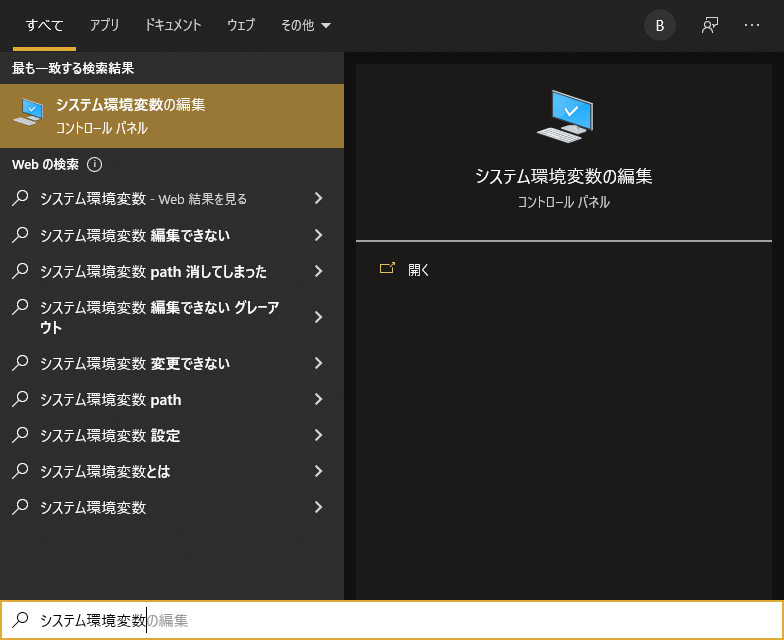
\includegraphics[width=8cm]{img/cmd-08-a.png}
\vspace{3mm}

``スタートボタン''を右クリックして「システム」を選択 --- 関連設定「システムの詳細設定」 でも
このウィンドウを開くことができる。


\vspace{3mm}
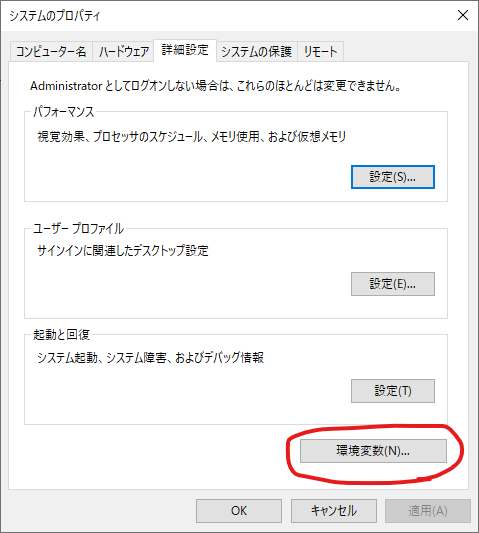
\includegraphics[width=8cm]{img/cmd-08.png}
\vspace{3mm}

開いたウィンドウで、``環境変数'' をクリックする。

環境変数のダイアログが開くので、``システム環境変数''の ``Path'' を
選択し、``編集''をクリックする。

\vspace{3mm}
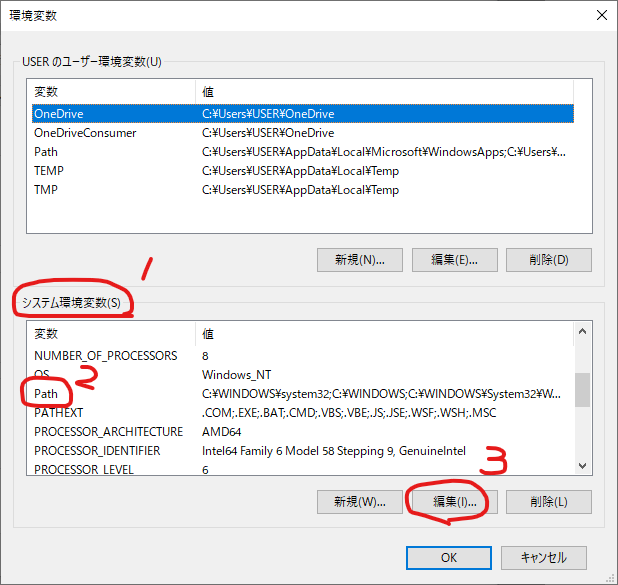
\includegraphics[width=8cm]{img/cmd-09.png}
\vspace{3mm}


環境変数名の編集ダイアログが開くので、``新規''を選択する。

\vspace{3mm}
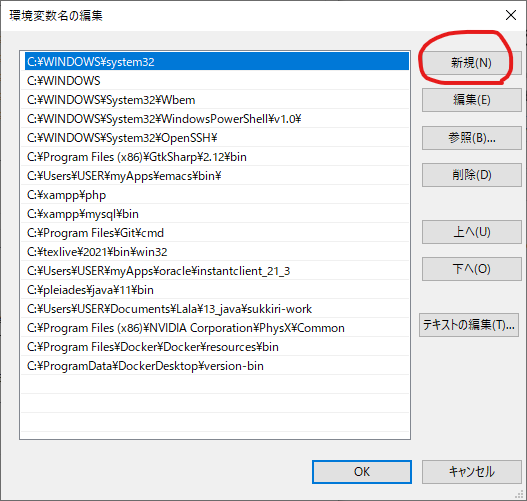
\includegraphics[width=8cm]{img/cmd-10.png}
\vspace{3mm}

入力欄ができる。``参照''をクリックする。

\vspace{3mm}
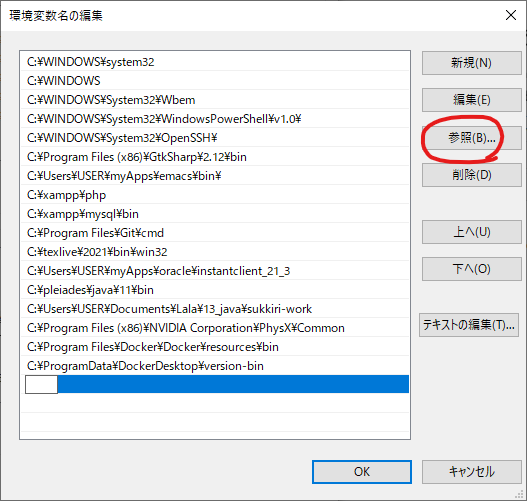
\includegraphics[width=8cm]{img/cmd-11.png}
\vspace{3mm}

開いたダイアログで デスクトップの ``myApp'' を選択して ``OK''。

\vspace{3mm}
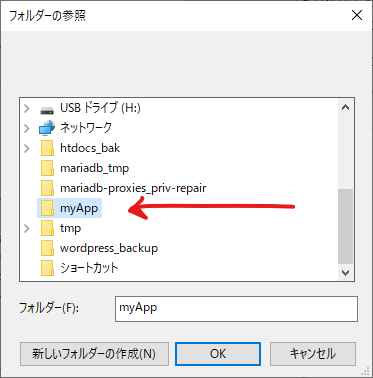
\includegraphics[width=8cm]{img/cmd-12.png}
\vspace{3mm}

``C:\yen Users\yen USER\yen Desktop\yen myApp'' が環境変数''Path'' に
登録された。

\vspace{3mm}
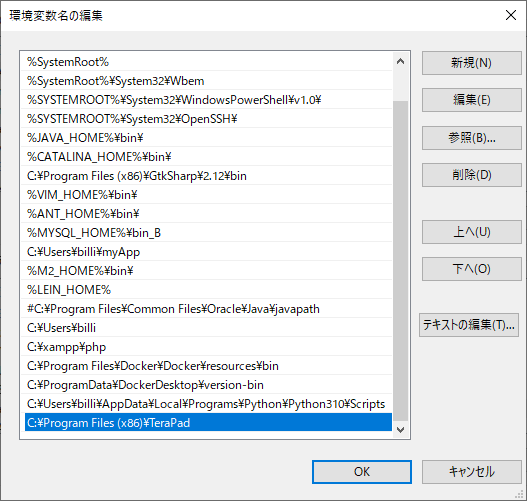
\includegraphics[width=8cm]{img/cmd-13.png}
\vspace{3mm}

あとは、``OK''をクリックしてダイアログを閉じていく。
``X''(閉じる)をクリックすると、今までの操作がすべてキャンセルされるので
気をつける。

このように システム環境変数の``Path'' にアプリのある場所を登録することで、
その場所にいなくても、そのアプリを実行できるようになる。

ただ、現在開いているコマンドプロンプトはいったん閉じて、
再度開きなおさないとこの変更は反映されない。


\vspace{3mm}
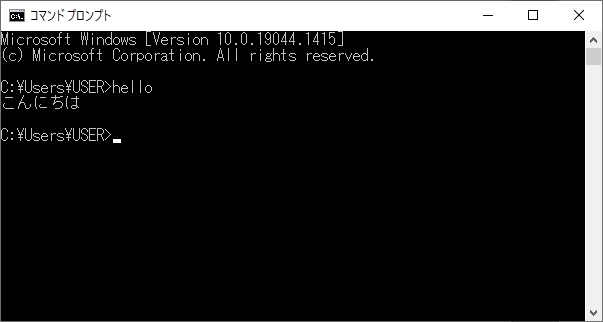
\includegraphics[width=12cm]{img/cmd-14-hello.png}
\vspace{3mm}

\newpage
\section{いろいろな情報}

\subsection{環境変数を画面に出力する}

``echo'' というコマンドがある。これは 画面出力したいときに使う。

たとえば、システム環境変数の ``PATH'' に何が登録されているかを調べるには、

\fbox{path}

と入力すると表示されるが、以下のようにすることもできる。

\fbox{echo \ \%path\%}

\% ではさんで echo すると、その変数の内容を出力することができる。

``HOME'' というシステム環境変数がある。
これにはユーザーのホームフォルダ(ホームディレクトリ)の位置(パス)がおさめられている。

\fbox{echo \ \%home\%}

とすると、その内容が表示される。また、

\fbox{cd \ \%home\%}

とすることで、他のディレクトリ(フォルダ)にいても、瞬時にホームディレクトリ(ホームフォルダ)に
戻ってこられる。

\fbox{set}

と入力すると、現在の環境変数が一覧できる。また、

\fbox{set \ home}

としても、環境変数 HOME の内容を確認できる。


\subsection{画面に出力された内容を保存する}

画面に出力された内容を保存することもできる。正確にいうと、echo の出力先を''画面''から
``ファイル''に変更することになる。

\fbox{echo \ \%path\% \ $>$ \ path.txt}

とすると、環境変数PATH の内容が path.txt に保存される。

\fbox{dir \ $>$ \ dir.txt}

とすると、``dir''で表示される内容を ``dir.txt'' というファイルに保存できる。

ただ、このコマンドを実行している場所(ディレクトリあるいはフォルダ) に保存される。
``C:\yen Users\yen USER''(ホーム)で実行しているなら、その場所に保存される。

システム環境変数の一覧を見たい場合も

\fbox{set \ $>$ \ set.txt}

とすると、set.txt をエディタで開き、システム環境変数の一覧を見ることができる。

\subsection{画面の出力を1ページずつにする}

たとえば \fbox{set} というコマンドを実行すると、システム環境変数の一覧が画面の上に流れていくが、

\fbox{set \ | \ more}

とすると、画面の高さによって、自動的に出力が停止し、画面下部に \fbox{-\-- more -\--} と
表示される。

ここで、``スペースキー'' を押すと、次の1画面高さ分表示される。

また、``Enterキー'' を押すと、1行ずつ上にずれて表示される。

``q'' を押すと、画面出力の MORE表示から抜けることができる。

\subsection{役に立つ(かもしれない)コマンド}

\subsubsection{ポート番号を調べる}

開発をしていると、ApacheなどのWebサーバーを80番ポートで動作させたいことがある。
ところが、80番ポートを他のアプリがすでに使っていて、Apacheを起動できない場合がある。
そんな時、80番ポートを使っているアプリを探すのに、以下のコマンドが役に立つ。

\fbox{netstat \ -noa}

画面上に流れていくから、

\fbox{netstat \ -noa \ $>$ \ netstat.txt}

とすると、エディタを使ってゆっくり見ることができる。また、

\fbox{netsata \ -noa \ | \ more}

とすると、1画面高さ分ずつ見ることができる。

``PID''とはプロセスIDのことで、これは''タスクマネージャー''をみることで そのプロセスIDは何の
アプリかはわかる。

あるいは、コマンドプロンプトを管理者権限で起動すると

\fbox{netstat \ -nba}

というコマンドが実行できる。これは、``PID''の代わりに、実行しているファイル名がわかる。

コマンドプロンプトを管理者権限で起動するには、スタートパネルから起動するとして、
そのアイコンを右クリックし、表示されたメニューから ``その他'' を選択し、
そのサブメニューから ``管理者として実行'' を選択するとよい。

\vspace{3mm}
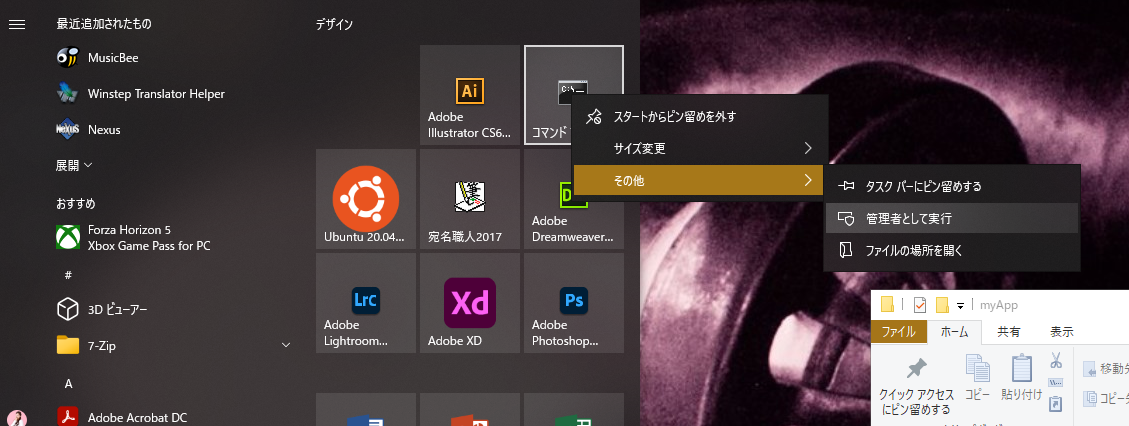
\includegraphics[width=15cm]{img/cmd-15.png}
\vspace{3mm}


\subsection{IPアドレスを調べる}

\subsubsection{自機のIPアドレスを調べる}

コンピュータのIPアドレスを調べることができる。

\fbox{ipconfig}

Wifiを使用しているなら、``Wireless LAN adapter Wi-Fi'' の項目を見る。

``IPv4 アドレス'' なら、``192.168.X.X''になっているはずである。(X はなにかの数字)

``デフォルト ゲートウェイ'' は、おそらく ``192.168.0.1''あるいは''192.168.1.1''に
なっているだろう。

\subsubsection{インターネット上のサイトのIPアドレスを調べる}

\fbox{nslookup \ google.co.jp} --- グーグルの場合

調べたいドメインを引数として入力すれば、nameサーバーに問い合わせてくれる。









\end{document}

%% 修正時刻: Sat May  2 15:10:04 2020


%% 修正時刻: Fri 2022/08/12 09:34:322
